\chapter{Applications}
\label{chap:applications}

\begin{figure}[ht]
	\hfill
	\begin{minipage}{0.5\textwidth}
		\centering
		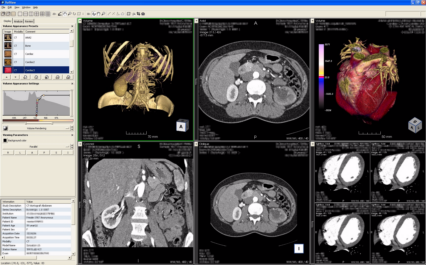
\includegraphics{VTKTextbook-275}
		\caption*{\texttt{Streamline visualization with ParaView Enterprise Edition.}}
	\end{minipage}
\end{figure}


\firstletter{W}e have described the design and implementation of an extensive toolkit of visualization techniques.
In this chapter we examine several case studies to show how to use these tools to gain insight into important application areas.
These areas are medical imaging, financial visualization, modeling, computational fluid dynamics, finite element analysis, and algorithm visualization. For each case, we briefly describe the problem domain and what information we expect to obtain through visualization.
Then we craft an approach to show the results.
Many times we will extend the functionality of the Visualization Toolkit with application specific tools.
Finally, we present a sample program and show resulting images.
The visualization design process we go through is similar in each case.
First, we read or generate application-specific data and transform it into one of the data representation types in the Visualization Toolkit.
Often this first step is the most difficult one because we have to write custom computer code, and decide what form of visualization data to use.
In the next step, we choose visualizations for the relevant data within the application.
Sometimes this means choosing or creating models corresponding to the physical structure. Examples include spheres for atoms, polygonal surfaces to model physical objects, or computational surfaces to model flow boundaries.
Other times we generate more abstract models, such as isosurfaces or glyphs, corresponding to important application data.
In the last step we combine the physical components with the abstract components to create a visualization that aids the user in understanding the data.

\section{3D Medical Imaging}
Radiology is a medical discipline that deals with images of human anatomy.
These images come from a variety of medical imaging devices, including X-ray, X-ray Computed Tomography (CT), Magnetic Resonance Imaging (MRI), and ultrasound. Each imaging technique, called an imaging modality, has particular diagnostic strengths.

\section{Bibliographic Notes}

The case studies presented in the chapter rely on having interesting data to visualize. Sometimes the hardest part of practicing visualizing is finding relevant data. The Internet is a tremendous resource for this task. Paul Gilste \cite{Gilster94} has written an excellent introduction to many of the tools for accessing information on the Internet. There are many more books available on this subject in the local bookstore.

In the stock case study we used a programming tool called AWK to convert our data into a form suitable for VTK. More information on AWK can be found in \emph{The AWK Programming Language} \cite{Aho88}. Another popular text processing languages is Perl \cite{Perl95}.

If you would like to know more about information visualization you can start with the references listed here \cite{Becker95} \cite{Ding90} \cite{Eick93} \cite{Feiner88} \cite{Johnson91} \cite{Robertson91}. This is a relatively new field but will certainly grow in the near future.

\printbibliography

\section{Exercises}

\begin{enumerate}

	\item The medical example did nothing to transform the original data into a standard coordinate system. Many medical systems use RAS coordinates. R is right/left, A is anterior/posterior and S is Superior/Inferior. This is the patient coordinate system. Discuss and compare the following alternatives for transforming volume data into RAS coordinates. See (\href{https://lorensen.github.io/VTKExamples/site/Cxx/VisualizationAlgorithms/AnatomicalOrientation/}{AnatomicalOrientation.cxx}) and (\href{https://lorensen.github.io/VTKExamples/site/Python/VisualizationAlgorithms/AnatomicalOrientation/}{AnatomicalOrientation.py}).
	\begin{enumerate}
		\item vtkActor transformation methods.
		\item vtkTransformFilter.
		\item Reader transformations.
	\end{enumerate}

	\item Modify the last example found in the medical application (\href{https://lorensen.github.io/VTKExamples/site/Cxx/Medical/Medical3/}{Medical3.cxx}) and (\href{https://lorensen.github.io/VTKExamples/site/Python/Medical/Medical3/}{Medical3.py}) to use vtkImageDataGeometryFilter instead of
	vtkImageActor. Compare the performance of using geometry with using
	texture. How does the performance change as the resolution of the
	volume data changes?

	\item Modify the last medical example (\href{https://lorensen.github.io/VTKExamples/site/Cxx/Medical/Medical3/}{Medical3.cxx}) to use vtkTexture and vtkPlaneSource instead of vtkImageActor.

	\item Change the medical case study to use dividing cubes for the skin surface.

	\item Combine the two scripts frogSegmentation.tcl and marchingFrog.tcl into one script that will handle either segmented or grayscale files. What other parameters and pipeline components might be useful in general for this application?

	\item Create polygonal / line stroked models of your initials and build your own logo. Experiment with different transformations.

	\item Enhance the appearance of Towers of Hanoi visualization.
	\begin{enumerate}
		\item Texture map the disks, base plane, and pegs.
		\item Create disks with central holes.
	\end{enumerate}

	\item Use the blow molding example as a starting point for the
	following.
	\begin{enumerate}
		\item Create an animation of the blow molding sequence. Is it possible to interpolate between time steps? How would you do this?
		\item Create the second half of the parison using symmetry. What   transformation matrix do you need to use?
	\end{enumerate}

	\item Start with the stock visualization example presented in this chapter.
	\begin{enumerate}
		\item Modify the example code to use a ribbon filter and linear extrusion filter as described in the text. Be careful of the width of the   generated ribbons.
		\item Can you think of a way to present high/low trade values for each day?
	\end{enumerate}

\end{enumerate}
